\documentclass[11pt,a4paper]{article}
\usepackage[margin=2cm]{geometry}
\usepackage{graphicx}
\usepackage{float}
\usepackage{booktabs}
\usepackage{tabularx}
\usepackage{xcolor}
\usepackage{listings}
\usepackage{tikz}
\usepackage[colorlinks=true,linkcolor=blue,urlcolor=blue]{hyperref}

\lstset{basicstyle=\ttfamily\footnotesize,breaklines=true,frame=single,
        backgroundcolor=\color{gray!8},columns=fullflexible,keepspaces=true}
\setlength{\parindent}{0pt}
\setlength{\parskip}{0.5em}
\graphicspath{{../../evidence/phase2/}}
\newcolumntype{Y}{>{\raggedright\arraybackslash}X}

% \shot{width}{file}{caption}
\newcommand{\shot}[3]{%
\begin{figure}[H]\centering
\includegraphics[width=#1\linewidth,height=0.30\textheight,keepaspectratio]{#2}
\caption{#3}\end{figure}}

\title{Computer Networks Course Project\\[2pt]
\large Phase 2: Harden, Recover and Troubleshoot -- Team 1}
\author{Vikrant Yadav (Mac 1) \quad Asad Ali (Mac 2)\\ Mayank Pillai (Mac 3) \quad Prashant Raj (Mac 4)}
\date{}

\begin{document}
\sloppy
\maketitle

% ============================================================
\section{Overview}

Phase 2 extends the Phase 1 network: we did not rebuild anything. A client still resolves
\texttt{app.team1.test} through our own DNS, connects over HTTPS to the nginx edge on port 8443, and
nginx load-balances to two Python backends. Phase 2 adds a backup DNS server, a 30-second DNS TTL,
firewall rules that isolate the backends, a tested backend failover, and a standby edge that we can
move traffic to by changing DNS. All tests were run on 22 November 2026.

The machine roles are the same as in Phase 1. Phase 2 only adds jobs. Both new services (the backup
DNS and the standby edge) have to run on a Mac other than Mac 1 and Mac 2, so they are on Mac 3.

\begin{table}[H]
\centering
\small
\begin{tabularx}{\linewidth}{llYYl}
\toprule
Mac & Member (Enrollment No.) & Phase 1 role (unchanged) & Added in Phase 2 & IPv4 \\
\midrule
1 & Vikrant Yadav (2401010504) & Primary DNS (dnsmasq)          & TTL 30 s on records                  & 10.7.29.164 \\
2 & Asad Ali (2401010108)      & nginx edge, TLS, load balancer & \texttt{X-Edge} header               & 10.7.26.179 \\
3 & Mayank Pillai (2401010268) & Backend A (3001) + client      & Backup DNS, standby edge, pf on 3001 & 10.7.18.13 \\
4 & Prashant Raj (2401010340)  & Backend B (3002) + client      & pf on 3002                           & 10.7.26.134 \\
\bottomrule
\end{tabularx}
\caption{Roles and the IP addresses used in Phase 2. The Wi-Fi (DHCP) gave every Mac a new address
since Phase 1, so all configuration takes its IPs from one file, \texttt{scripts/team.env}.}
\end{table}

\begin{figure}[H]
\centering
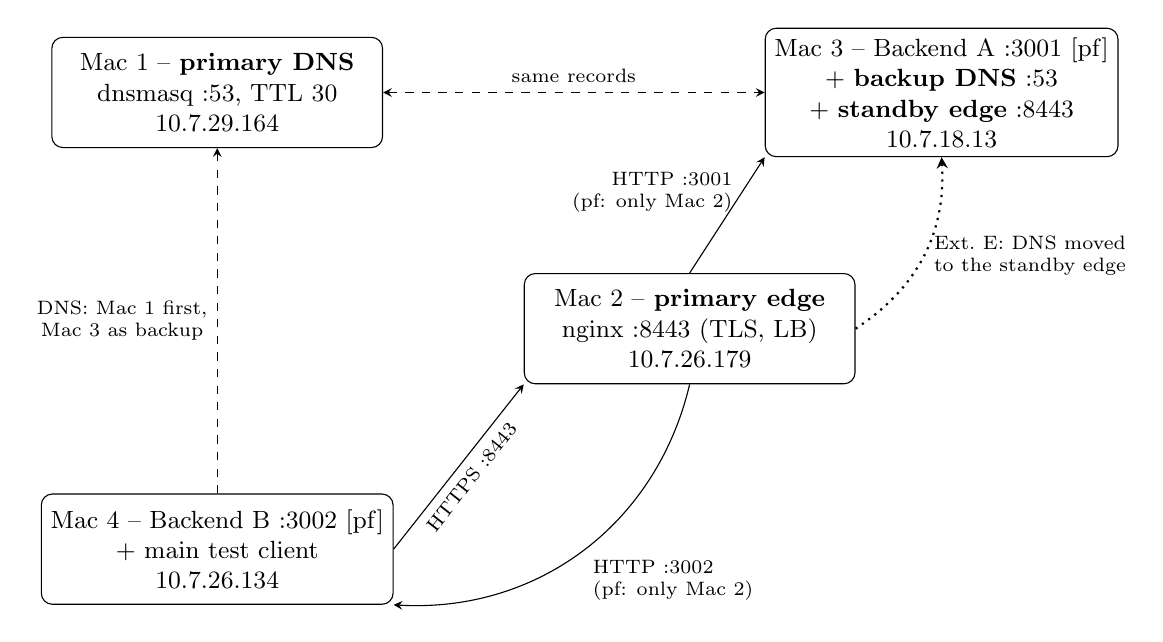
\begin{tikzpicture}[box/.style={draw,rounded corners,minimum width=4.2cm,minimum height=1.4cm,align=center,font=\small},
                    >=stealth]
\node[box] (dns)  at (-4.6,2.6) {Mac 1 -- \textbf{primary DNS}\\dnsmasq :53, TTL 30\\10.7.29.164};
\node[box] (m3)   at (4.6,2.6)  {Mac 3 -- Backend A :3001 [pf]\\+ \textbf{backup DNS} :53\\+ \textbf{standby edge} :8443\\10.7.18.13};
\node[box] (edge) at (1.4,-0.4)   {Mac 2 -- \textbf{primary edge}\\nginx :8443 (TLS, LB)\\10.7.26.179};
\node[box] (m4)   at (-4.6,-3.2){Mac 4 -- Backend B :3002 [pf]\\+ main test client\\10.7.26.134};
\draw[<->,dashed] (dns) -- node[above,font=\scriptsize]{same records} (m3);
\draw[->,dashed] (m4) -- node[left,font=\scriptsize,align=center]{DNS: Mac 1 first,\\Mac 3 as backup} (dns);
\draw[->] (m4.east) -- node[below,sloped,font=\scriptsize]{HTTPS :8443} (edge.south west);
\draw[->] (edge.north) -- node[left,font=\scriptsize,align=right,pos=0.7]{HTTP :3001\\(pf: only Mac 2)} (m3.south west);
\draw[->] (edge.south) to[bend left=40] node[below right,font=\scriptsize,align=left,pos=0.5]{HTTP :3002\\(pf: only Mac 2)} (m4.south east);
\draw[->,dotted,thick] (edge.east) to[bend right=30] node[right,font=\scriptsize,align=left]{Ext.\ E: DNS moved\\to the standby edge} (m3.south);
\end{tikzpicture}
\caption{Phase 2 topology. Dashed: DNS. Solid: HTTPS and proxied HTTP. [pf]: firewall rule.}
\end{figure}

% ============================================================
\section{What Changed from Phase 1}

\begin{table}[H]
\centering
\small
\begin{tabularx}{\linewidth}{lYY}
\toprule
Part & Phase 1 & Phase 2 \\
\midrule
DNS servers & One server (Mac 1) & Primary on Mac 1 and a backup on Mac 3 with identical records \\
DNS records & \texttt{address=...}: answers sent with TTL 0, so clients never cache &
  \texttt{host-record=...,30}: TTL 30 s, so clients cache for up to 30 s \\
DNS forwarding & Read \texttt{/etc/resolv.conf} & \texttt{no-resolv} + \texttt{server=8.8.8.8}, to avoid a loop now that the
  DNS servers' own Macs may list the team DNS servers \\
Client resolver & Mac 1 only & Mac 1 first, Mac 3 second (\texttt{networksetup -setdnsservers}) \\
Backend access & Any machine on the LAN could open port 3001/3002 & pf allows only the edge (10.7.26.179); everyone else is dropped \\
nginx edge & TLS, round robin, \texttt{max\_fails}/\texttt{fail\_timeout}, \texttt{proxy\_next\_upstream} &
  Same, plus an \texttt{X-Edge} response header and the new backend IPs \\
Edge redundancy & None & Standby nginx on Mac 3 with the same config and the same mkcert certificate; traffic moved by DNS \\
Operations & Configured by hand & One script per member (\texttt{scripts/}) that backs up every file before changing it and can roll back \\
\bottomrule
\end{tabularx}
\end{table}

\subsection*{Configuration}
Primary DNS (Mac 1). The backup on Mac 3 is identical except for \texttt{listen-address=10.7.18.13}:
\lstinputlisting{../../config/phase2/dnsmasq-mac1-primary.conf}

Firewall rule on Mac 3 (Mac 4 is the same with port 3002), loaded with \texttt{pfctl -f}:
\lstinputlisting{../../config/phase2/pf-mac3-backend-a.conf}

nginx: the only changes to the Phase 1 edge config are the backend addresses and one header line
(\texttt{config/phase2/nginx-mac2-primary.conf}; the standby copy says \texttt{standby-mac3}):
\begin{lstlisting}
upstream backend_servers {
    server 10.7.18.13:3001 max_fails=1 fail_timeout=10s;  # Mac 3 (Backend A)
    server 10.7.26.134:3002 max_fails=1 fail_timeout=10s; # Mac 4 (Backend B)
}
...
        add_header X-Edge "primary-mac2" always;   # Phase 2: shows which edge answered
\end{lstlisting}

% ============================================================
\section{Resilience Tests and Results}

\begin{table}[H]
\centering
\small
\begin{tabularx}{\linewidth}{lYYl}
\toprule
Ext. & Test & Result & Status \\
\midrule
A & Stop dnsmasq on Mac 1; client resolves and opens the site & Primary timed out, backup answered, site HTTP 200 & Passed \\
B & Change the record, then check cache vs DNS; flush & New answer after the TTL; flush gave the change at once & Passed \\
C & pf on both backends; connect from edge and from clients & Edge ALLOWED, clients BLOCKED (timeout), site still 200; rollback done & Passed \\
D & Stop Backend A during load & 6/6 requests HTTP 200 from B; A rejoined after restart & Passed \\
E & Standby edge on Mac 3, move DNS, stop the primary & Clients moved to \texttt{standby-mac3}; site worked with the primary stopped & Passed \\
\bottomrule
\end{tabularx}
\caption{Summary of the Phase 2 resilience tests.}
\end{table}

% ------------------------------------------------------------
\subsection{Extension A: Backup DNS resolver}

\textbf{Setup.} Both DNS servers return \texttt{app.team1.test -> 10.7.26.179} with TTL 30. Mac 3 and
Mac 4 list 10.7.29.164 first and 10.7.18.13 second.

\shot{0.85}{extA-backup-dns/02-mayank-backup-dns-answers}{Backup DNS on Mac 3 answers with the same record as the primary.}
\shot{0.85}{extA-backup-dns/01-vikrant-primary-dns-ttl30}{Primary DNS on Mac 1 written with TTL 30 and answering for \texttt{app.team1.test}.}
\shot{0.6}{extA-backup-dns/03-prashant-client-uses-both-dns-servers}{Client (Mac 4) is configured with both DNS servers, primary first.}
\shot{0.6}{extA-backup-dns/04-mayank-client-uses-both-dns-servers}{Second client (Mac 3) is configured with both DNS servers.}
\shot{0.75}{extA-backup-dns/05-prashant-both-dns-servers-answer}{21:08:49: both DNS servers answer the client with 10.7.26.179, TTL 30.}

\textbf{Test.} We stopped dnsmasq on Mac 1 (\texttt{brew services stop dnsmasq}). At 21:10:26 the
client's queries gave:
\begin{lstlisting}
ERR DNS server 10.7.29.164 did not answer for app.team1.test
;; connection timed out; no servers could be reached
OK  DNS server 10.7.18.13 answers:
app.team1.test.         30      IN      A       10.7.26.179
== What this Mac itself uses (system resolver, can fail over) ==
OK  app.team1.test -> 10.7.26.179
\end{lstlisting}
(full output: \texttt{extA-backup-dns/terminal-prashant-primary-dns-down.txt}). With the primary still
stopped, the site returned HTTP 200:
\shot{0.7}{extA-backup-dns/06-prashant-site-works-while-primary-dns-down}{21:15:41, primary DNS stopped: HTTPS request still succeeds (served by Backend B).}
\shot{0.6}{extA-backup-dns/07-prashant-loop-after-backends-restarted}{21:29:50: after the DNS and backend tests, normal load balancing across A and B.}

\textbf{DNS failure vs application failure.} When the DNS service fails, the problem is name resolution:
\texttt{dig} to that server times out, and nothing after it can start. When an application server fails,
resolution still works: \texttt{dig} returns 10.7.26.179, TCP and TLS to the edge succeed, and the
failure only shows at HTTP level as a \texttt{502 Bad Gateway} from nginx
(Figure~\ref{fig:502} in Section~\ref{sec:trouble} shows such a 502).

% ------------------------------------------------------------
\subsection{Extension B: DNS TTL and controlled record change}

\textbf{Setup.} Records are served with TTL 30 (second column of the \texttt{dig} answer). In Phase 1
the TTL was 0, so clients could not cache answers at all.

\textbf{Test.} The client first resolved the name (cached \texttt{10.7.26.179}). Both DNS servers then
changed the record to 10.7.26.134 (\texttt{point-to mac4}). The client's \texttt{check-cache} command
prints two answers: (1) the macOS resolver, which uses the cache, and (2) a fresh \texttt{dig}, which does not.

\shot{0.85}{extB-ttl/01-mayank-point-to-mac4}{Record changed to 10.7.26.134 on the backup DNS (the same change on the primary).}
\shot{0.75}{extB-ttl/02-prashant-check-cache-213229-new-ip}{21:32:29: after the TTL, cached and fresh answers are both the new IP.}
\shot{0.75}{extB-ttl/03-prashant-check-cache-213333-new-ip}{21:33:33: the client keeps resolving the new IP.}
\shot{0.85}{extB-ttl/04-mayank-point-back-to-mac2}{Record changed back to the edge, 10.7.26.179.}

We then changed the record back to 10.7.26.179 and flushed the client cache
(\texttt{dscacheutil -flushcache; killall -HUP mDNSResponder}). The new answer was used immediately,
without waiting for the TTL:
\shot{0.75}{extB-ttl/05-prashant-flush-changes-immediately}{21:35:01: after a flush the client gets the changed record at once.}

\textbf{Relation to production.} Before migrating a service, operators lower the TTL well in advance.
After the record is changed, clients move within one TTL; the old server must keep running until
then, because clients with a cached answer still go to it.

% ------------------------------------------------------------
\subsection{Extension C: Service isolation with backend firewall rules}

\textbf{Setup.} On Mac 3 and Mac 4 we loaded a pf ruleset that passes TCP to the backend port only
from the edge (10.7.26.179) and silently drops it from everyone else. The original
\texttt{/etc/pf.conf} is never edited; a copy is also kept in \texttt{\textasciitilde/.team1-phase2/}.

\shot{0.9}{extC-firewall/01-mayank-firewall-on-port-3001}{pf rules active on Mac 3 (port 3001).}
\shot{0.9}{extC-firewall/02-prashant-firewall-on-port-3002}{pf rules active on Mac 4 (port 3002).}
\shot{0.9}{extC-firewall/03-asad-edge-allowed-to-both-backends}{From the edge (Mac 2), both backends are reachable.}
\shot{0.9}{extC-firewall/05-prashant-direct-to-backend-a-blocked}{From a client (Mac 4), a direct connection to Backend A is blocked.}
\shot{0.9}{extC-firewall/04-mayank-direct-to-backend-b-blocked}{From the other client (Mac 3), a direct connection to Backend B is blocked.}
\shot{0.6}{extC-firewall/06-prashant-site-works-through-edge-with-firewall-on}{21:40:47, firewall on: the site still works through the edge, A and B alternating.}

While the rules were on, the site still worked through the edge (A and B alternating at 21:40:47,
\texttt{extC-firewall/06}). We then rolled back with \texttt{pfctl -f /etc/pf.conf} and disabled pf,
which had been off before:
\shot{0.7}{extC-firewall/07-mayank-firewall-off-rollback}{Rollback on Mac 3: only Apple's default anchors remain.}
\shot{0.7}{extC-firewall/08-prashant-firewall-off-rollback}{Rollback on Mac 4.}

\textbf{Observation.} A blocked connection \emph{times out}, because pf drops the SYN without replying.
A stopped service answers with a TCP reset, so the client sees \emph{connection refused} immediately.
The difference tells us whether a firewall or a dead process is the cause.

% ------------------------------------------------------------
\subsection{Extension D: High-availability failover}

nginx uses \emph{passive} health checks: \texttt{max\_fails=1 fail\_timeout=10s} marks a backend as down
for 10 s after one failed attempt, and \texttt{proxy\_next\_upstream error timeout} retries the same request
on the other backend, so the client does not see the error.

\shot{0.6}{extD-failover/01-prashant-both-backends-a-b}{21:43:31: normal round robin.}
\shot{0.6}{extD-failover/02-prashant-backend-a-down-all-b-200}{21:44:24: Backend A stopped; all six requests succeed from B.}
\shot{1.0}{extD-failover/03-asad-nginx-log-retry-a-to-b}{nginx access log. At 21:44:25 one request shows
\texttt{upstream=10.7.18.13:3001, 10.7.26.134:3002}: it was sent to A, failed, and was retried on B.
Later requests go straight to B while A is marked down.}
\shot{0.6}{extD-failover/04-prashant-backend-a-back-a-b}{21:46:31: Backend A restarted; both backends serve requests again.}

\textbf{Remaining single point of failure.} The edge nginx on Mac 2. If it stops, no client can reach
the service, even though both backends are healthy. Extension E shows one way to recover (moving DNS
to a standby edge), but it is manual and clients wait up to one TTL. Removing the single point of
failure needs two edges that share a floating IP (VRRP with keepalived, so the standby takes over the
same IP in seconds), or health-checked DNS failover (like Route 53 failover records), or a managed,
redundant load balancer (AWS ALB). The Wi-Fi access point is also a single point of failure, and so
is Mac 3, which now carries Backend A, the backup DNS and the standby edge.

% ------------------------------------------------------------
\subsection{Extension E: Controlled edge migration (DNS-based cutover)}

\textbf{Setup.} Mac 3 runs a second nginx with the same configuration and the same mkcert certificate
for \texttt{app.team1.test}, copied from Mac 2 (the private key was sent only by AirDrop and is not in
Git). Both edges add an \texttt{X-Edge} header, so the client can see which edge answered.

\shot{0.85}{extE-edge-cutover/02-mayank-standby-edge-ready}{Standby edge on Mac 3: valid TLS, HTTP 200, \texttt{x-edge: standby-mac3}.}
\shot{0.85}{extE-edge-cutover/01-asad-x-edge-primary-header}{Primary edge on Mac 2 now labels its replies \texttt{x-edge: primary-mac2}.}

\textbf{Cutover.} At 21:59:02 the client used the primary edge. Both DNS servers then changed
\texttt{app.team1.test} to 10.7.18.13. At 21:59:58 the client was on the standby edge, and a client with
an empty cache (Mac 3, after a flush) went to the standby immediately.

\shot{0.75}{extE-edge-cutover/03-prashant-before-cutover-primary-edge}{21:59:02: before the change, the primary edge (Mac 2) answers.}
\shot{0.85}{extE-edge-cutover/05-vikrant-point-to-mac3}{Primary DNS moves \texttt{app.team1.test} to the standby edge (the backup DNS did the same).}
\shot{0.85}{extE-edge-cutover/04-mayank-point-to-mac3}{Backup DNS moves \texttt{app.team1.test} to the standby edge.}
\shot{0.75}{extE-edge-cutover/06-prashant-after-ttl-standby-edge}{21:59:58: the client now reaches the standby edge.}
\shot{0.75}{extE-edge-cutover/07-mayank-fresh-lookup-standby-edge}{22:00:44: a client with an empty cache (Mac 3, after a flush) resolves straight to the standby edge.}
\shot{0.75}{extE-edge-cutover/08-prashant-standby-edge-again}{22:01:20: the client is still served by the standby edge.}
\shot{0.75}{extE-edge-cutover/09-asad-primary-edge-stopped}{nginx on the primary edge (Mac 2) is stopped.}

With the primary stopped, the service kept working through the standby only:
\shot{0.75}{extE-edge-cutover/10-prashant-service-works-on-standby-only}{22:04:55: primary edge stopped; all requests HTTP 200 via \texttt{standby-mac3}, both backends used.}

Finally we moved DNS back to Mac 2, restarted the primary, and stopped the standby:
\shot{0.85}{extE-edge-cutover/11-mayank-point-back-to-mac2}{DNS points \texttt{app.team1.test} back to the primary edge.}
\shot{0.75}{extE-edge-cutover/12-asad-primary-edge-restarted}{Primary edge restarted: \texttt{x-edge: primary-mac2}.}
\shot{0.75}{extE-edge-cutover/13-prashant-back-on-primary-edge}{22:09:36: after a flush the client is back on the primary edge.}
\shot{0.6}{extE-edge-cutover/14-mayank-standby-edge-stopped}{Standby nginx on Mac 3 stopped.}

\textbf{TTL effects.} With a 30 s TTL, a client that resolved the name less than 30 s before the change
keeps using its cached address, so it still reaches the old edge until the answer expires. A client
with no cached answer (Mac 3 after a flush) goes to the standby at once. For a real migration the old
edge therefore has to stay up for at least one TTL after the record is changed.

% ============================================================
\section{Troubleshooting Findings}
\label{sec:trouble}

The faculty-injected fault (Extension F) happens at the evaluation. During the Phase 2 session we
found and fixed several real faults, all with the same layer-by-layer method: name resolution
(\texttt{dig}), then IP reachability (\texttt{ping}), then TCP (\texttt{nc -vz}), then TLS and HTTP
(\texttt{curl -v}), then the backends directly from the edge.

\begin{table}[H]
\centering
\small
\begin{tabularx}{\linewidth}{YYYY}
\toprule
Symptom & What the checks showed & Cause (layer) & Fix \\
\midrule
New setup: nothing worked with the Phase 1 config & \texttt{ipconfig getifaddr en0} gave a new IP on every Mac &
  DHCP had given new addresses (network) & One shared \texttt{team.env}; DNS records, nginx upstream and pf rules regenerated from it \\
\texttt{curl} to the site: exit 7 / timeout & DNS OK; ping to Mac 2 OK; \texttt{nc} to 8443 timed out; \texttt{lsof} showed nginx on 80 and 8080 only &
  nginx was running Homebrew's default config, not the edge config (transport / service) & Installed the edge config, restarted nginx \\
HTTP 502 after about 4 s & DNS, TCP and TLS OK; \texttt{grep server} in nginx.conf showed the Phase 1 backend IPs &
  Stale upstream addresses (application: edge to backend) & Updated the upstream IPs, \texttt{nginx -s reload} \\
Script: \texttt{bind() to 0.0.0.0:8443 failed (Address already in use)} & Config valid; a second nginx was started &
  Our script started instead of reloading (service) & \texttt{nginx -s reload}; script fixed to reload first \\
Backup DNS check failed once right after setup & A query a few seconds later succeeded & dnsmasq still starting (DNS) & Script now retries for 10 s \\
Requests sometimes timed out & DNS OK; ping RTT to Mac 2 was 150--870 ms; later the same request connected in 6 ms &
  Congested Wi-Fi (link / network) & Longer timeouts in the scripts; kept Mac 2 awake and close to the access point \\
\bottomrule
\end{tabularx}
\end{table}

\shot{0.7}{extF-troubleshooting/01-prashant-502-stale-backend-ips-in-nginx}{\label{fig:502}HTTP 502: the edge answered (DNS, TCP and TLS
worked) but could not reach any backend. It took about 4 s because nginx tried each stale backend IP
for its 2 s \texttt{proxy\_connect\_timeout}.}
\shot{0.85}{extF-troubleshooting/02-prashant-dns-ok-but-edge-timeout}{DNS answers from both servers, but TCP to the edge times out:
the fault is below HTTP, at the edge's TCP port.}

The terminal output for the nginx diagnosis is saved as \texttt{terminal-asad-nginx-diagnosis.txt} in the \texttt{extF-troubleshooting} folder.
Mac 2 is a managed Mac whose macOS application firewall cannot be changed from the command line. We
checked that this firewall was not the cause: closed ports on Mac 2 returned \emph{connection refused}
(a TCP reset) instead of timing out, so packets were not being silently dropped.

After all tests, every Mac was back to its normal state: firewalls off, standby stopped, DNS pointing
at Mac 2. (Mac 2's last line shows \texttt{[--]} only because Mac 2 is not a test client and does not
use the team DNS.)
\shot{0.75}{extF-troubleshooting/03-mayank-status-all-ok}{Final status of Mac 3.}
\shot{0.65}{extF-troubleshooting/04-prashant-status-all-ok}{Final status of Mac 4.}
\shot{0.65}{extF-troubleshooting/05-asad-status}{Final status of Mac 2.}

% ============================================================
\section{Learning Summary}

\textbf{Extension A (backup DNS).} Name resolution is its own service and can fail on its own. With
two resolvers configured, the client's resolver moved to the backup after the primary timed out, and
the user did not notice. We learned to tell a DNS failure (the name cannot be resolved, \texttt{dig}
times out) from an application failure (the name resolves, TCP and TLS work, but HTTP returns 502), and
that both DNS servers must always hold the same records.

\textbf{Extension B (TTL).} The TTL is a promise about how long an answer may be reused. With TTL 0 in
Phase 1 every lookup reached our server; with TTL 30 the client kept using its cached answer, and a
cache flush made it ask again at once. This is why a DNS change is never instant, and why production
teams lower the TTL before a migration and keep the old server alive for one TTL afterwards.

\textbf{Extension C (service isolation).} A backend that only the edge can reach can only be used
through the edge, where TLS, logging and load balancing happen. pf rules are evaluated per packet, so
we allowed the edge's IP first and then dropped everything else. We also learned to read the symptom:
a firewall drop gives a timeout, a stopped service gives connection refused, and keeping a rollback
(the untouched \texttt{/etc/pf.conf}) makes such changes safe.

\textbf{Extension D (HA failover).} nginx's passive health checks were enough to hide a backend crash
from users: the failed request was retried on Backend B, and Backend A was skipped for 10 seconds and
then used again automatically. Redundant backends do not remove the single point of failure in front
of them; the edge itself must be duplicated (floating IP or DNS failover).

\textbf{Extension E (edge migration).} Moving the edge needed nothing on the clients: only a DNS
change, because clients only know the name. The standby needed the same configuration and the same
certificate, since TLS validates the name, not the IP. The cost of DNS-based cutover is the TTL
window, during which clients with a cached answer still go to the old edge.

\textbf{Extension F (troubleshooting).} The real faults we met (new DHCP addresses, nginx running the
wrong config, stale upstream IPs, a slow Wi-Fi) were found fastest by checking one layer at a time:
\texttt{dig}, \texttt{ping}, \texttt{nc}, \texttt{curl -v}, then the edge's own logs and config. The
first check that fails points to the broken layer; for example, a 502 means DNS, TCP and TLS are fine
and the problem is between the edge and the backends.

% ============================================================
\section{Where to Find Everything}
\begin{itemize}
\item Evidence, one folder per extension, with an index: \texttt{evidence/phase2/README.md}
\item Phase 2 configuration bundle: \texttt{config/phase2/} (Phase 1 files in \texttt{config/} are unchanged)
\item Scripts and the step-by-step run order: \texttt{scripts/README.md}
\item Topology and roles: \texttt{docs/ARCHITECTURE.md}
\end{itemize}

\end{document}
